\section{Mapping victims with Telescopes and Honeypot}\label{sec:mapping_victim}
This analysis establish a relationship between our recorded DDOS event data and the Telescopes and  Honeypots datasets. It specifically focuses on aligning full-day dates, spanning from midnight to the end of the day, with our defined intervals of DDOS events, as marked by startTime and endTime. 
In Telescopes' operational design, attacks are detected by analyzing backscattered traffic. This traffic typically results from attack traffic that spoofs its source address to resemble that of the Telescopes' address blocks. Based on this detection method, we can anticipate two primary scenarios:
Due to our mitigation mechanisms, there is only a slim chance that the date recorded by Telescopes will coincide with our event dataset. If Telescopes record a date that precedes the startTime and endTime of a DDOS event, it might be indicative of an attack being detected early by the Telescopes. Following this early detection, mitigation measures might be activated within the DDOS event window to address the attack. On the other hand, if a date recorded by Telescopes falls after the DDOS event timeframe, it could imply a re-emergence of the attack, occurring after the mitigation measures detailed in the DDOS event data.
The Honeypots dataset, however, provides a contrasting perspective. Unlike Telescopes, Honeypots are not just detection tools; they actively participate in attack mechanisms. As such, their data might align with DDOS events by coincidence. The occurrence of a Honeypot record during a DDOS event does not inherently suggest a direct link with the event's mitigation processes, as Honeypots operate independently of these countermeasures
\begin{figure}[htbp]
    \centering
    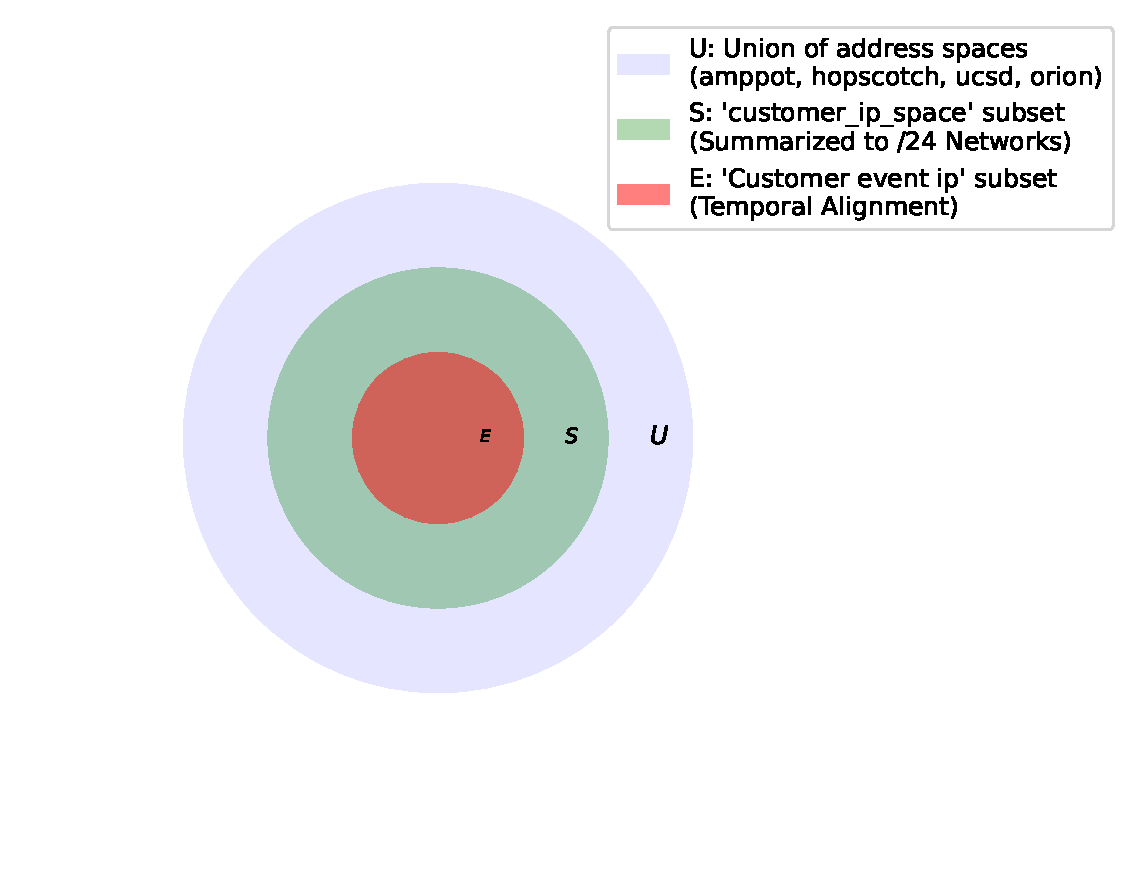
\includegraphics[scale=0.5]{graphs/sets.pdf}
    \caption{Address sets relationship}
    \label{fig:addresssets}
\end{figure}

\subsection*{'customer\_ip\_space' Definition}
\begin{figure}[htbp]
    \centering
    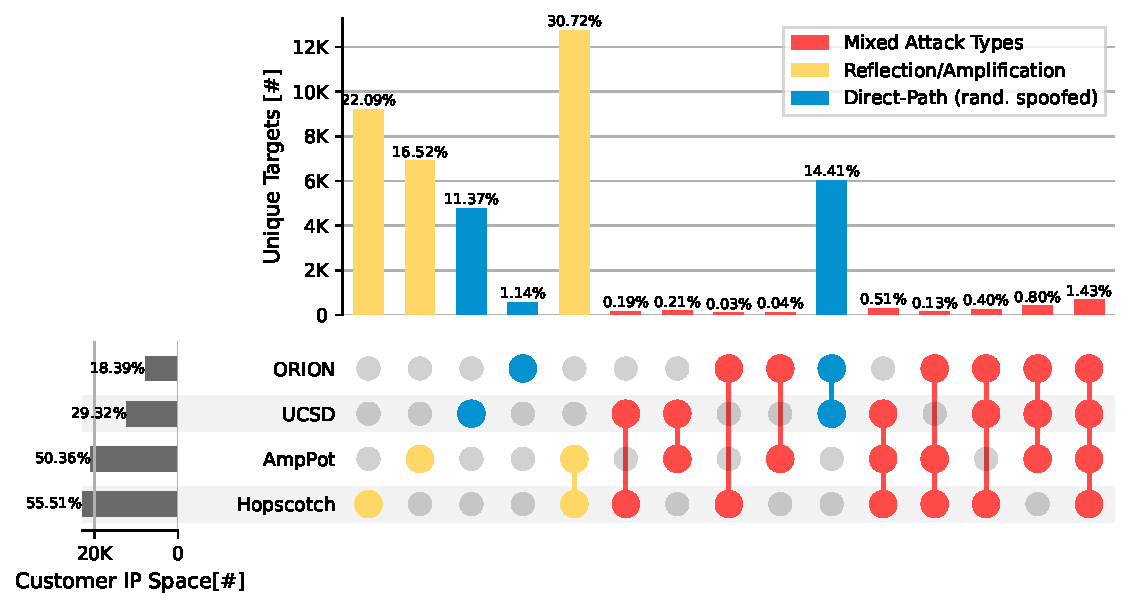
\includegraphics[scale=0.4]{graphs/space_no_event.pdf}
    \caption{Customer IP Space Analysis.}
    \label{fig:customeripspace}
\end{figure}
Fig. \ref{fig:customeripspace} shows the attack event detected by telescopes and honeypots for our interested ip space $S$.
    
Let $U$ represent the union of address spaces from the categories 'amppot', 'hopscotch', 'ucsd', and 'orion'. The 'customer\_ip\_space' condition identifies a subset of $U$, denoted as $S$, characterized by the following criteria:
\begin{enumerate}
    \item \textbf{Summarization to Class C Networks}: Each IP address in $S$ is summarized to a Class C network, represented by the first three octets of the IP address, effectively transforming the address into a /24 network notation.
    \item \textbf{Match with Summarized /24 Networks}: An address $s \in S$ is considered part of 'customer\_ip\_space' if its summarized /24 network matches with any summarized /24 network within $U$.
\end{enumerate}

\subsection*{'Customer event ip' Definition}
\begin{figure}[htbp]
    \centering
    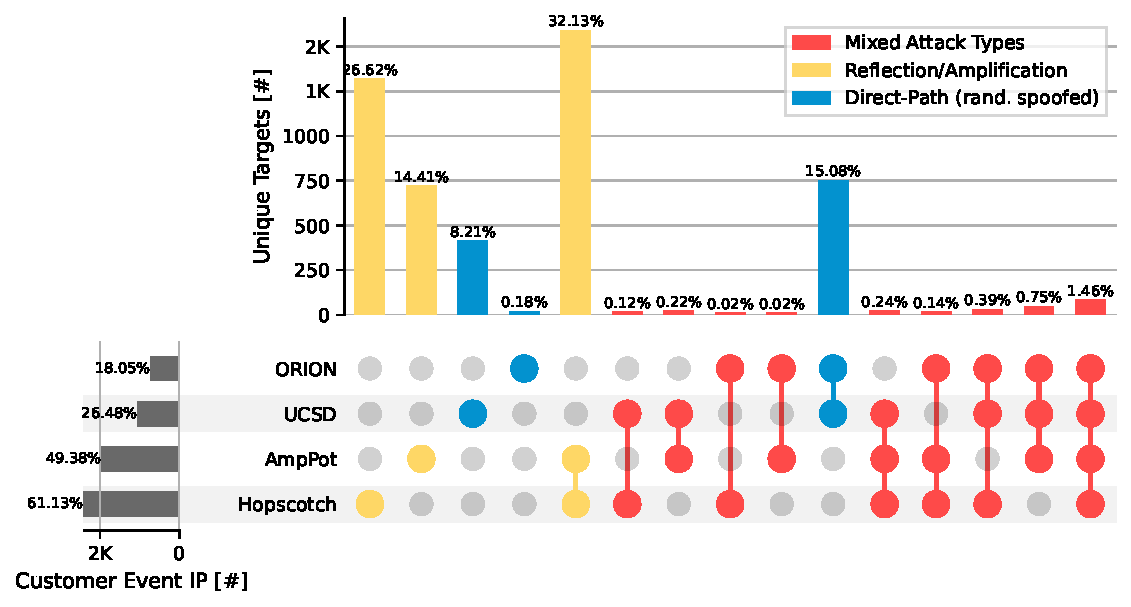
\includegraphics[scale=0.4]{graphs/space_event.pdf}
    \caption{Customer Event IP Analysis.}
    \label{fig:customereventip}
\end{figure}
Fig. \ref{fig:customereventip} shows the attack event detected by telescopes and honeypots for our interested ip attack events $S$.


The 'Customer event ip' condition extends the identification of relevant IP addresses by incorporating temporal alignment with specific events. It represents a subset of 'customer\_ip\_space', denoted as $E$, with the following additional condition:

\begin{enumerate}
    \item \textbf{Temporal Alignment with Events}: For an address $e \in E$, not only must it satisfy the 'customer\_ip\_space' criteria, but it must also coincide with an event whose duration ($p$) matches a specified date ($d$). The event duration is defined by the start and end times of activity associated with the IP address. An event is considered to match if $d$ falls within this duration, indicating that the event occurred within the specified timeframe.
\end{enumerate}
Fig. \ref{fig:addresssets} shows relationship among the $U$ $S$ $E$.

\begin{figure}[htbp]
    \centering
    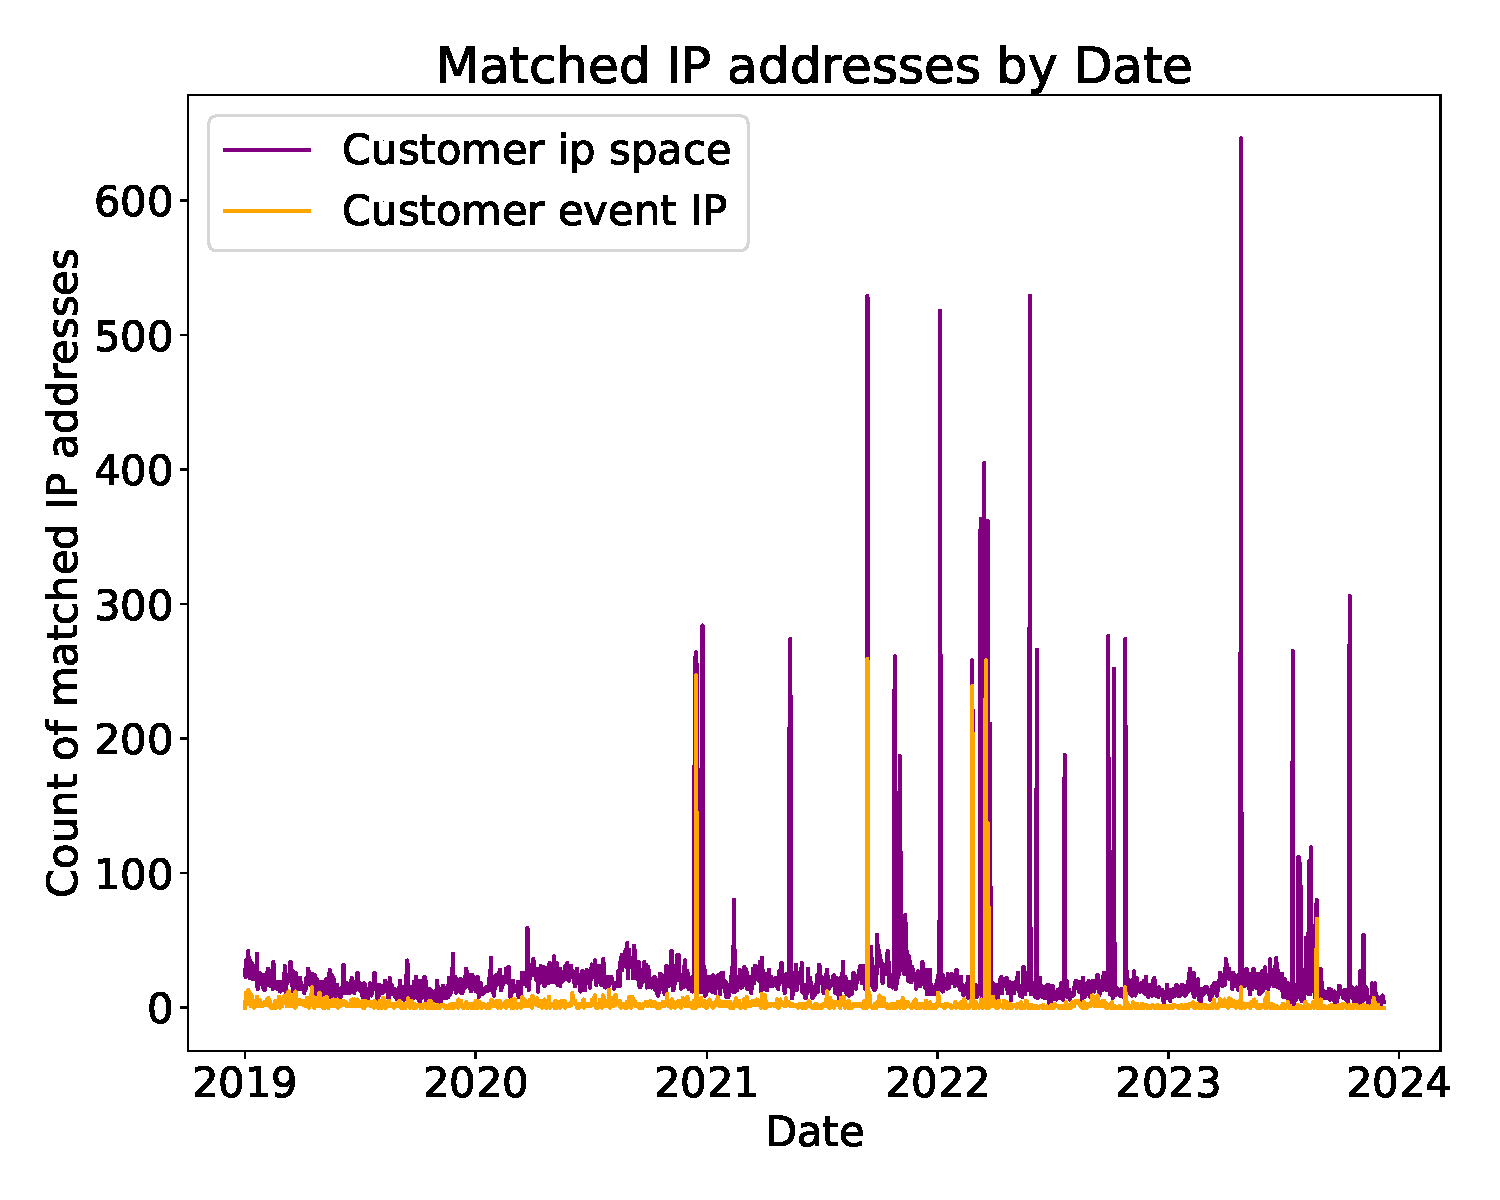
\includegraphics[scale=0.30]{graphs/matched_customer_graph.pdf}
    \caption{Mapping customer ip space and event.}
    \label{fig:mappedcustomergraph}
\end{figure}

\begin{figure*}[htbp]
    \centering
    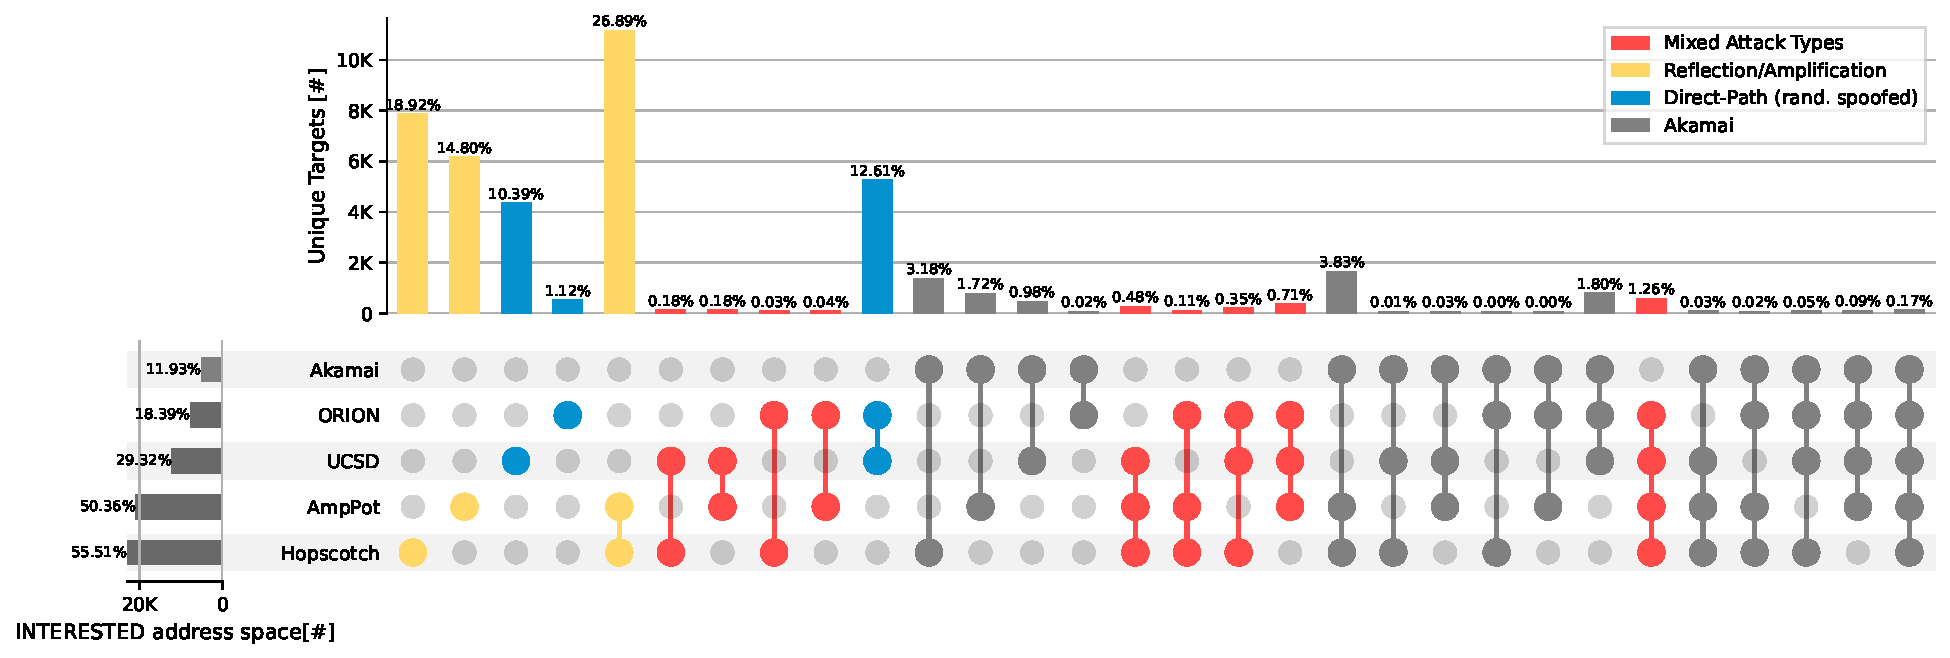
\includegraphics[scale=0.48]{graphs/noir3.pdf}
    \caption{Customer IP Space and event Analysis.}
    \label{fig:Mappedaddressanalysis}
\end{figure*}

\section{Attack Incidents Analysis}\label{sec:attackeventsfromcustomeripspace}
Fig. \ref{fig:mappedcustomergraph} visualizes the count of matched IP addresses over time, distinguishing between "Customer IP Space" and "Customer Event IP". It shows spikes indicating significant events: (A) a large number of targets detected from the Customer IP Space by telescopes/honeypots and (B) a large number of targets from Customer (Attacks) Events recorded by the DPS.

\subsection{Spikes detected by Telescopes and Honeypots}
\begin{itemize}
    \item \textbf{Telescope Detection:} Telescopes identifies spoofed attacks targeted at IP subnets, manifested as backscattered traffic. It is observed in two specific scenarios: 
    \begin{enumerate}
        \item When a customer transitions to DDoS Protection Services (DPS) for mitigation.
        \item Prior to the effectiveness of DPS mitigation measures.
    \end{enumerate}
    
    \item \textbf{Honeypot Detection:} Honeypots detect both direct and reflection attacks, actively engaging with all IP addresses within the targeted subnets.
\end{itemize}

\begin{table*}[htbp]
    \centering
    \caption{Matched IP counts showed as spikes in Fig \ref{fig:mappedcustomergraph}}
    \begin{tabular}{|l|l|r|r|r|r|r|}
    \hline
    \textbf{Date} & \textbf{Victim Subnet} & \textbf{Amppot} & \textbf{Hopscotch} & \textbf{UCSD} & \textbf{Orion} & \textbf{Akamai} \\
    \hline
    2020-12-15 & Subnet A & 83 & 246 & 0 & 0 & 246 \\
    2021-09-12 & Subnet B & 0 & 0 & 256 & 256 & 256 \\
    2022-02-25 & Subnet C & 1 & 1 & 239 & 0 & 239 \\
    2022-03-18 & Subnet D & 1 & 256 & 1 & 1 & 256 \\
    2022-03-22 & Subnet D & 0 & 135 & 1 & 1 & 135 \\
    2023-08-24 & Subnet E & 0 & 0 & 66 & 66 & 66 \\
    \hline
    \end{tabular}
    \label{table:splits_data}
    \end{table*}


The data from the telescopes, which aligns with our DDOS events, is vividly represented by the spikes 
Customer IP Space in this context identifies IP addresses of our customers that are detected and logged within the telescopes/honeypot datasets. The designation Customer Event IP, however, is more specifically applied to those customer IPs that not only appear in the telescopes/honeypot datasets but also coincide with the broader timeframes delineated by the \texttt{startTime} and \texttt{endTime} of our DDOS events. Crucially, this correlation is not based on exact hour, minute, and second details, since the telescopes/honeypot data does not include these precise time elements. Rather, matching is determined by the day, with the assumption that each recorded date encompasses the full 24-hour span from one midnight to the next.
